\chapter{Architecture}
\label{chap:num_4}

The following chapter provides the overview of the architecture of \lpas. Explains the main components of the Storage as well as how it is being integrated into LinkedPipes Applications platform.

\section{High level overview}

While the majority of components were described in detail in chapter  \ref{chap:num_1}, the overview architecture provided in this section shows more specific details on how all the external and internal components of the system are interacting. One of the essential details represented in the figure \ref{fig:lpas_high_level_architecture} is the separation between codebases of \lpa{} and \lpas{}. The \lpa{} Frontend is imports the \lpas{} as an npm package and performs all interactions with Solid using the provided functionality of the package. In some sense, \lpas{} is being threated as an additional rudimentary backend and database layer on top of existing internal components inside \lpa{}. This is due to several functional requirements that \lpas{} package implements,  such as \textit{user authentication}, \textit{storage crud operations} and etc.

\begin{figure}[h]
\centering
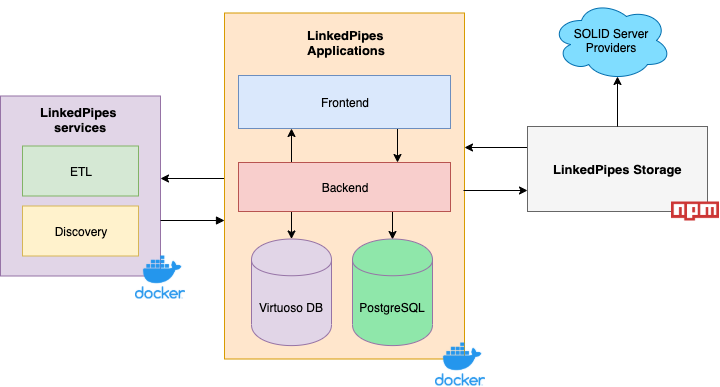
\includegraphics[width=14cm]{lpas_high_level_architecture.png}
\caption{High level overview of \lpa{} and \lpas{} interactions}
\label{fig:lpas_high_level_architecture}
\end{figure}

As additionally demonstrated, the figure \ref{fig:lpas_high_level_architecture} also has Docker icons displayed under some modules. This is to indicate where the production-ready service is hosted. For instance, in the case of the \lpas{}, the end goal is the npm registry, while \lps{} and \lpa{} are all hosted in the docker registry where each internal component is a docker container.
The generic interaction flow usually involves direct communication between the \lpa{} frontend and \lpas{} package. The internal frontend component have various React components implemented using the \lpas{} package that provide navigation and interaction with \solid{} Pods. While the package is designed under the assumption that the \lpa{} is the only user of the package, some abstractions are generic enough and have the potential to be used outside of the scope of the main functional requirements. The implementation chapter will also cover a generic use-case on how quick start with application development based on \solid{}.

\subsubsection{The evolution of solid specifications}

At the moment of writing this chapter, the official \solid{} specification reached version \texttt{0.7.0} \footnote{\url{https://github.com/solid/solid-spec/blob/master/CHANGELOG.md}}. Introducing many changes and improvements, it also adds an extra layer of complexity with every release, changing some of the conventions or updating some fundamental paradigms. As a result, when \lpa{} was initially implemented, it was based on an older specification and older versions of \texttt{NSS}, that had simpler and more extensive ability to manipulate \texttt{ACL} files. The work within this project however was focused around putting efforts into making it generic enough so that people could use it as a guideline for any started \solid{} apps, while the implementation will fit all \lpa{} requirements.

The main note to mention for the further section in this chapter is that the architecture design was derived with an aim to rely on official specification of \solid{} while also referring to the provided functionality of \texttt{NSS} that does not always strictly follow the guidelines in specification. 


\section{The Storage}

The initial architecture and implementation draft of \lpas{} were different from what is presented in this chapter.  \solid{} related logic was firstly a part of the \lpa{} codebase. Therefore, significantly complicating unit testing and making it hard to define the scopes of the \lpa{} and \lpas{} projects implementation. Later on, a decision was made to separate the logic of the \lpas{} and move it in the separate codebase. The majority of abstractions that were initially designed to be inside the \lpa{} codebase, consisted of various wrappers and crud functions to interact with \solid{} servers. Their design was refined and aggregated into specific abstractions, each responsible for covering the functional requirements from \lpa{} project.

\begin{figure}[h]
\centering
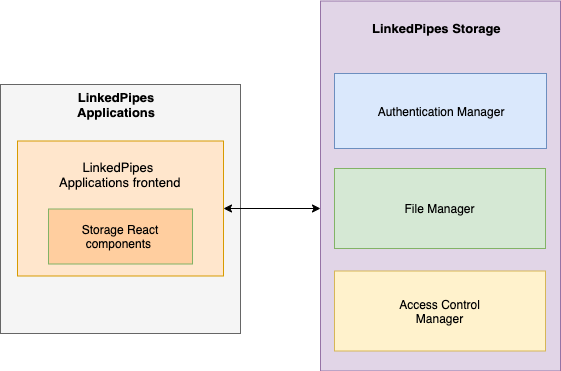
\includegraphics[width=14cm]{lpas_high_level_abstractions.png}
\caption{Main abstractions of \lpas.}
\label{fig:lpas_high_level_abstractions}
\end{figure}

Let us start by describing the main abstractions providing the functionality of \lpas{}.

\subsection{Authentication Manager}

The Authentication Manger is responsible for wrapping \solid{} \textit{WebID} based authentication logic into a simple and developer friendly abstraction. As already mentioned in chapter \ref{chap:num_3}, the usage of \textit{WebID} protocols is one of many benefits of \solid{}, in contrast with popular authentication protocols used in centralized silos, it is completely agnostic to specific authentication mechanisms, allowing our single abstraction to support any arbitrary \textit{WebID-OIDC} compliant \solid{} provider.

At the moment of writing this, the official \solid{} specification states to support the following protocols:
\begin{itemize}
\item WebID-TLS  - is one of the primary authentication protocols that relies on WebIDs instead of usernames. The passwords are replaced with certain cryptographic certificates as bearer tokens and is stored within user's browser.
\item WebID-OIDC - alternative authentication protocol based on OAuth2 and OpenID Connect protocols and adjusted to support the concept of WebID. This is in fact the primary authentication option provided by \lpas{}, later chapters will provide reasoning behind why this ended up being more intuitive option to cover the authentication requirement for \lpa{}.   
\end{itemize}

\subsubsection{Interacting with frontend}

Sequence diagram on figure \ref{fig:lps_authentication_sequence_diagram} demonstrate an example on how the Authentication Manager will be used within the \lpa{} Frontend and how it will interact with \solid{} Providers. The user agent entity represents a typical lay \lpa{} user interacting with the platform through the frontend component. The sequence flow consist of the following steps:

% TODO: cite the node-solid-server
\begin{enumerate}
    \item The user simply clicks on 'Authenticate' button. This is the starting point of this sequence diagram that serves as a trigger for \lpa{} to invoke the \lpa{} package.
    \item The frontend component calls the Authentication Manager and asynchronously awaits for a callback. As a main input it supplies the information about the \solid{} provider that user would like to use.
    \item The Authentication Manager contacts the \solid{} provider and requests the provider authentication web page. Each provider conforming to \solid{} specification should contain that page.
    \item Depending on the browser environment of the user, he gets redirected to the provider's authentication web page either in a new browser tab or a popup dialog.
    \item User selects the preferred authentication and inputs the credentials. At the moment of writing this thesis, popular \solid{} server implementations like node-solid-server support both WebID+TLS and WebID-OIDC specifications.
    \item The Authentication Manager receives the callback from the provider and sets the authenticated user session token.
    \item Frontend component receives the callback from the Authentication Manager indicating that user is authenticated.
    \item As a last step, frontend redirects the user into the homepage dashboard of \lpa{} platform.
\end{enumerate}


\begin{figure}[h]
\centering
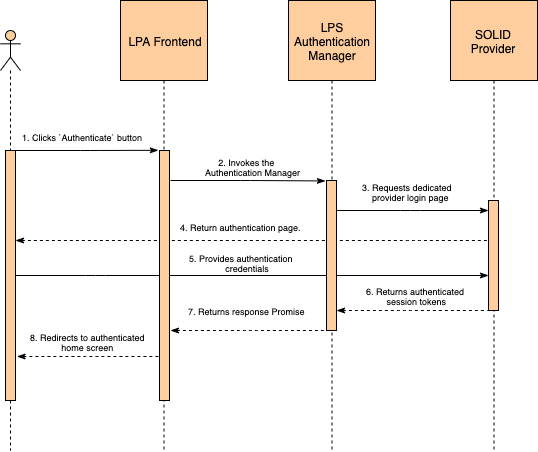
\includegraphics[width=12cm]{lps_authentication_sequence_diagram.png}
\caption{Sequence diagram for \textit{authenticate} operation invoked from \lpa{} frontend.}
\label{fig:lps_authentication_sequence_diagram}
\end{figure}


\subsection{File Manager}
% TODO: add citations
The File Manager is responsible for implementing the CRUD operations for the \solid{}  providers that are compliant with LinkedData Platform specification. The LinkedData Platform or LDP is a specification that is reused and extended in the \solid{} specification to describe the REST API for interacting with LDP Resources and LDP Containers. LDP Resources and LDP Containers are, in some sense, the basic building blocks of any \solid{} POD, since they allow users to create any files and folders. 

As mentioned earlier, \solid{} specification is re-using the LDP specification\footnote{https://www.w3.org/TR/ldp/} to provide a RESTful set of operations to interact with any compliant implementation of that specification. 

The LDP has an extensive set of resource types that are suited for defining the folder and files. However, the architecture provided is relying on two common resource terminologies that were simple enough to cover the requirements without complicating the design of the architecture. Those resources are defined as follows:

\begin{itemize}
%	Cite resource 
 	\item Linked Data Platform Basic Container (LDP-BC), is a Linked Data Platform Basic Container. A LDP-RS representing a collection of linked documents that responds to client requests for creation, modification, and/or enumeration of its linked members and documents, and that conforms to the simple lifecycle patterns and conventions.
	\item A HTTP resource whose state is represented in any way that conforms to the simple lifecycle patterns and conventions. The LDP servers process the CRUD operations to manipulate the lifecycle of LDPRs.
\end{itemize}


\subsubsection{Creating resources}

The most essential operation thats is at the core of most functional requirements defined earlier is the ability to create a resource in a POD. Using NSS server as a basis the general convention for creating LDP resources is a \texttt{POST} providing link to the POD under the path where resource need to be created. 

\subsubsection{Reading resources}

Reading the resources demonstrated on figure \ref{fig:lps_get_resource_sequence} is a straightforwards set of interactions with an \solid{} specification compliant server, and it can be described as follows:

\begin{enumerate}
    \item \lpa{} frontend invokes the FileManager abstraction with a request specified in \texttt{ResourceConfig} abstraction. The configuration provided contains information on the type of the resource, whether it is a folder or a file, as well as all required information to identify the resource within the POD.
    \item \lpas{} constructs an HTTP GET request to obtain the information from \solid{} server from the provider, the response is simply forwarded in asynchronous fashion.
\end{enumerate}

As demonstrated in steps above, the LDP specification provides advantages by narrowing down the amount of resource lifecycle related calls to as set of very simple CRUD operations. Another important detail is that every single resource created by \lpas{} is an RDF. We will cover more information and demonstrate why it is implemented in that way in the proceeding chapter.  
 
\begin{figure}[h]
\centering
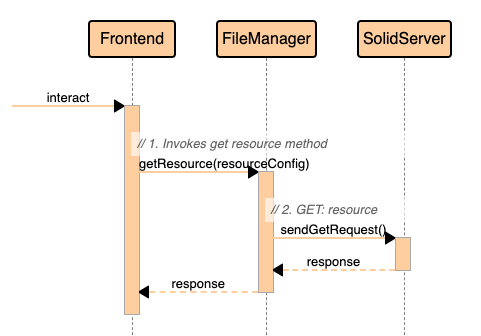
\includegraphics[width=10cm]{get_resource.png}
\caption{Sequence diagram for \textit{GET} resource operation invoked from StorageFileManager.}
\label{fig:lps_get_resource_sequence}
\end{figure}

\subsubsection{Renaming resources}

The rename operation covers one of the functional requirements on \lpa{} platform. It is based on some simpler CRUD operations described in earlier sections. The intent is to provide an ability for an \lpa{} developer to implement a functionality to let \lpa{} platform users to choose and manipulate their storage configuration folders. 

The flow on the sequence diagram displayed on figure \ref{fig:lps_rename_resource} consist of the following steps:

\begin{enumerate}
    \item \lpa{} frontend invokes the FileManager abstraction with a request specified in \texttt{ResourceConfig} abstraction, this is similar to input steps in previous sequence diagrams. 
    \item \lpas{} has a conditional check to see whether the new provided resource configuration is not accidentally the resource under same title. This step is followed if the new path and title for a configuration is not equal to an old configuration.
    	\begin{enumerate}
    	\item Invoke the copy method that will depending on the resource either will copy it directly, if it is a file, or copy it recursively if it is a folder. For a sake of reducing the unnecessary details, the internals of the copy resource call is not displayed on this diagram.
    	\item After copying the content of configuration into new destination, the old resource it removed using the delete operation.
    	\end{enumerate}
    \item \lpas{} returns a successful promise since no renaming is invoked in that case. 
\end{enumerate}

\begin{figure}[h]
\centering
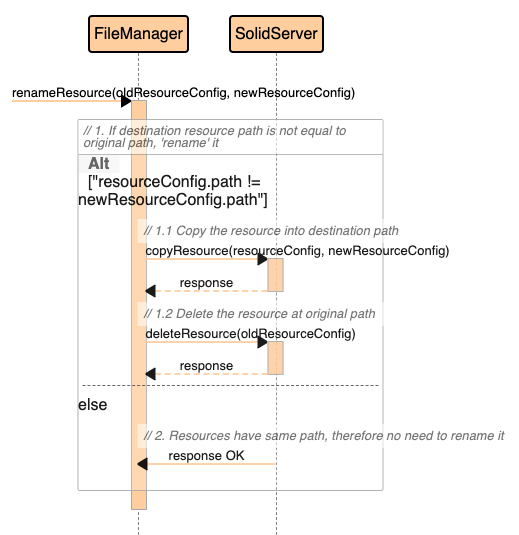
\includegraphics[width=10cm]{rename_resource.png}
\caption{Sequence diagram for a complex operation to rename a particular resource in StorageFileManager.}
\label{fig:lps_rename_resource}
\end{figure}

\subsubsection{Deleting resources}

Deletion of resources is slightly more complicated in comparison with trivial GET, POST, PUT or PATCH operations described in earlier sections. The main goal here is to differentiate the type of the resource and depending on whether it is an LDP Basic Container or generic LDP Resource, act accordingly to delete all files under that resource. 
The flow from figure \ref{fig:lps_delete_resource} can be described as follows:

\begin{enumerate}
    \item Similar to previous sequence flows, the action is triggered by an input request from \lpa{} frontend
    \item If resource is and LDP Resource, FileManager trivially sends 
   	a single DELETE request to the server and returns the response
    \item If resource is an LDP Basic Container:
    	\begin{enumerate}
    	\item Invokes a method for recursively deleting contents of a folder.
    	\item Within that method, it performs a call that fetches the raw RDF describing the LDP Basic Container and parses the resources contained within using. 
    	\item Iterate over files, remove the individually as in first step.
    	\item Iterate over folders, remove them individually as in first step 
    	\end{enumerate}
\end{enumerate}


\begin{figure}[h]
\centering
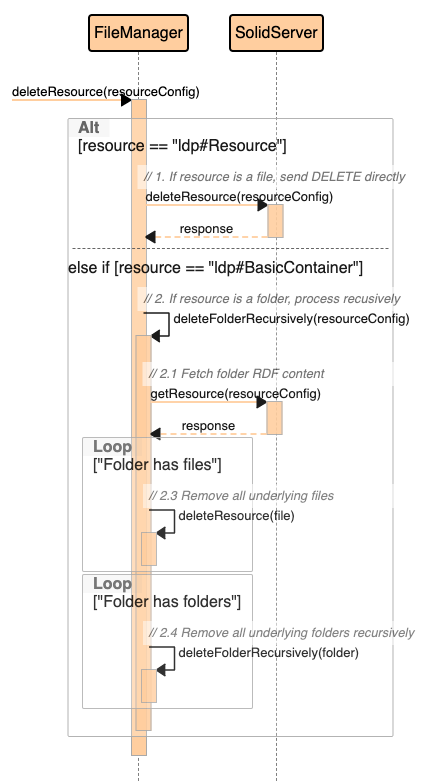
\includegraphics[width=8cm]{delete_resource.png}
\caption{Sequence diagram for a complex operation to delete a particular resource in StorageFileManager.}
\label{fig:lps_delete_resource}
\end{figure}


One of the assumption made in this recursive operation is the interactions with \texttt{ACL} files when recursive delete is performed. As mentioned in the introduction to this chapter, \solid{} community is still at its beginnings and there are many significant improvements yet to introduce. In order to make the delete operation more generic, the DELETE interactions with \texttt{ACL} files were have to be removed due to a more strict access policy established between providers of the server and \solid{} apps. The following section will dive deeper into Access Control Managements and related functionality.

\subsubsection{Classes overview}

File manager is the biggest of all three abstractions displayed on the figure \ref{fig:lpas_high_level_abstractions}. Therefore, in order to better describe the architecture of it, a more detail class diagram is provided on figure \ref{fig:lps_file_manager_class_uml}.

\begin{itemize}
	\item The core class available to \lpa{} developers is the \textit{StorageFileManager}. All of the functions inside are intended to be public, static and asynchronous. 
	\item \textit{ResourceConfiguration} is a wrapper for LDP Containers and LDP Resources. It allows a developer to specify \textit{title}, \textit{path} and \textit{type} of a resource. Most of the operations within the \textit{StorageFileManager} are operated with the resources encapsulated into \textit{ResourceConfiguration} classes. It also provides a few helper getters that allow to generate an absolute path to a resource within a pod. 
	\item The \textit{AccessControlConfig} is a subclass of \textit{ResourceConfig}. It allows to specify the access control modes to individual resources. Additionally, it introduces a few extra functions to generate the absolute path that includes the \texttt{.acl} extension.   
	\item The \textit{SolidResource} is a simple interface that includes various details specific to the resource. Some of the fields provided are also directly used by \textit{StorageFileManager} abstraction during construction of CRUD calls to \solid{} providers.
\end{itemize}


\begin{figure}[h]
\centering
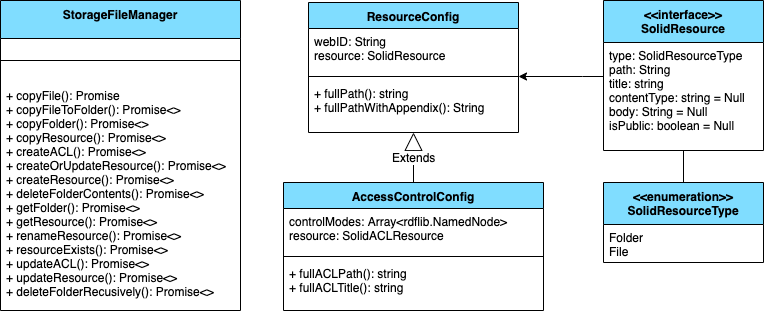
\includegraphics[width=14cm]{lpas_storage_file_manager_uml.png}
\caption{A higher level class diagram of classes contained within StorageFileManager abstraction.}
\label{fig:lps_file_manager_class_uml}
\end{figure}


\subsection{Access Control Manager}

The primary responsibility of the Access Control Manager is a subset under File Manager abstraction. It is designed to support the File Manager entities and provide an ability to wrap them with Web Access Control compliant settings. In other words, this allows a developer of \lpa{} to programmatically control the Read and Write access to any resource inside an arbitrary \solid{} POD by utilising the developer-friendly interfaces and classes defined within the scope of this abstraction. Essentially every \texttt{ACL} files is nothing more than yet another RDF resource with few extra features. Hence, the abstraction was placed under the File Manager since the core logic is concerned with similar resource lifecycle manipulations.
%TODO add citations

It is yet another wrapper on top of the functionality provided by any \solid{} compliant servers. In this case, being \solid{} compliant also assumes conforming to Web Access Control or WAC specification. It defines the so-called Access Control Resources, which are entities serving as the declaration of access control privileges for a specific resource. Within the context of \solid{} specification this means managing access rights to resources in \solid{} PODS for various WebIDs.

The main function provided by the abstraction is an acl file generator. The flow on the figure \ref{fig:lps_acl_update_flow} demonstrated the process of generation, parsing and serialization of ACL files: 

\begin{enumerate}
	\item Create Access Control triples for specified input resource configuration file.
	\item Create individual triples defining acl configuration for a resource owner.
	\item Create individual triples for public access, if the resource itself is marked as public.
	\item Gather and parse those triples into a an rdflib abstraction representing an RDF Graph.
	\item Serialize this graph instance into a string representing a \texttt{text/turtle} file.
	\item Finally perform an HTTP call, that uses PUT to create an ACL file attached to a specified resource.
\end{enumerate}

This concludes the section demonstrating the essential abstractions within the \lpas{} package. The consecutive chapters dedicated to Documentation will cover and provide more details regarding less significant classes and utilities available inside the package.

\begin{figure}[h]
\centering
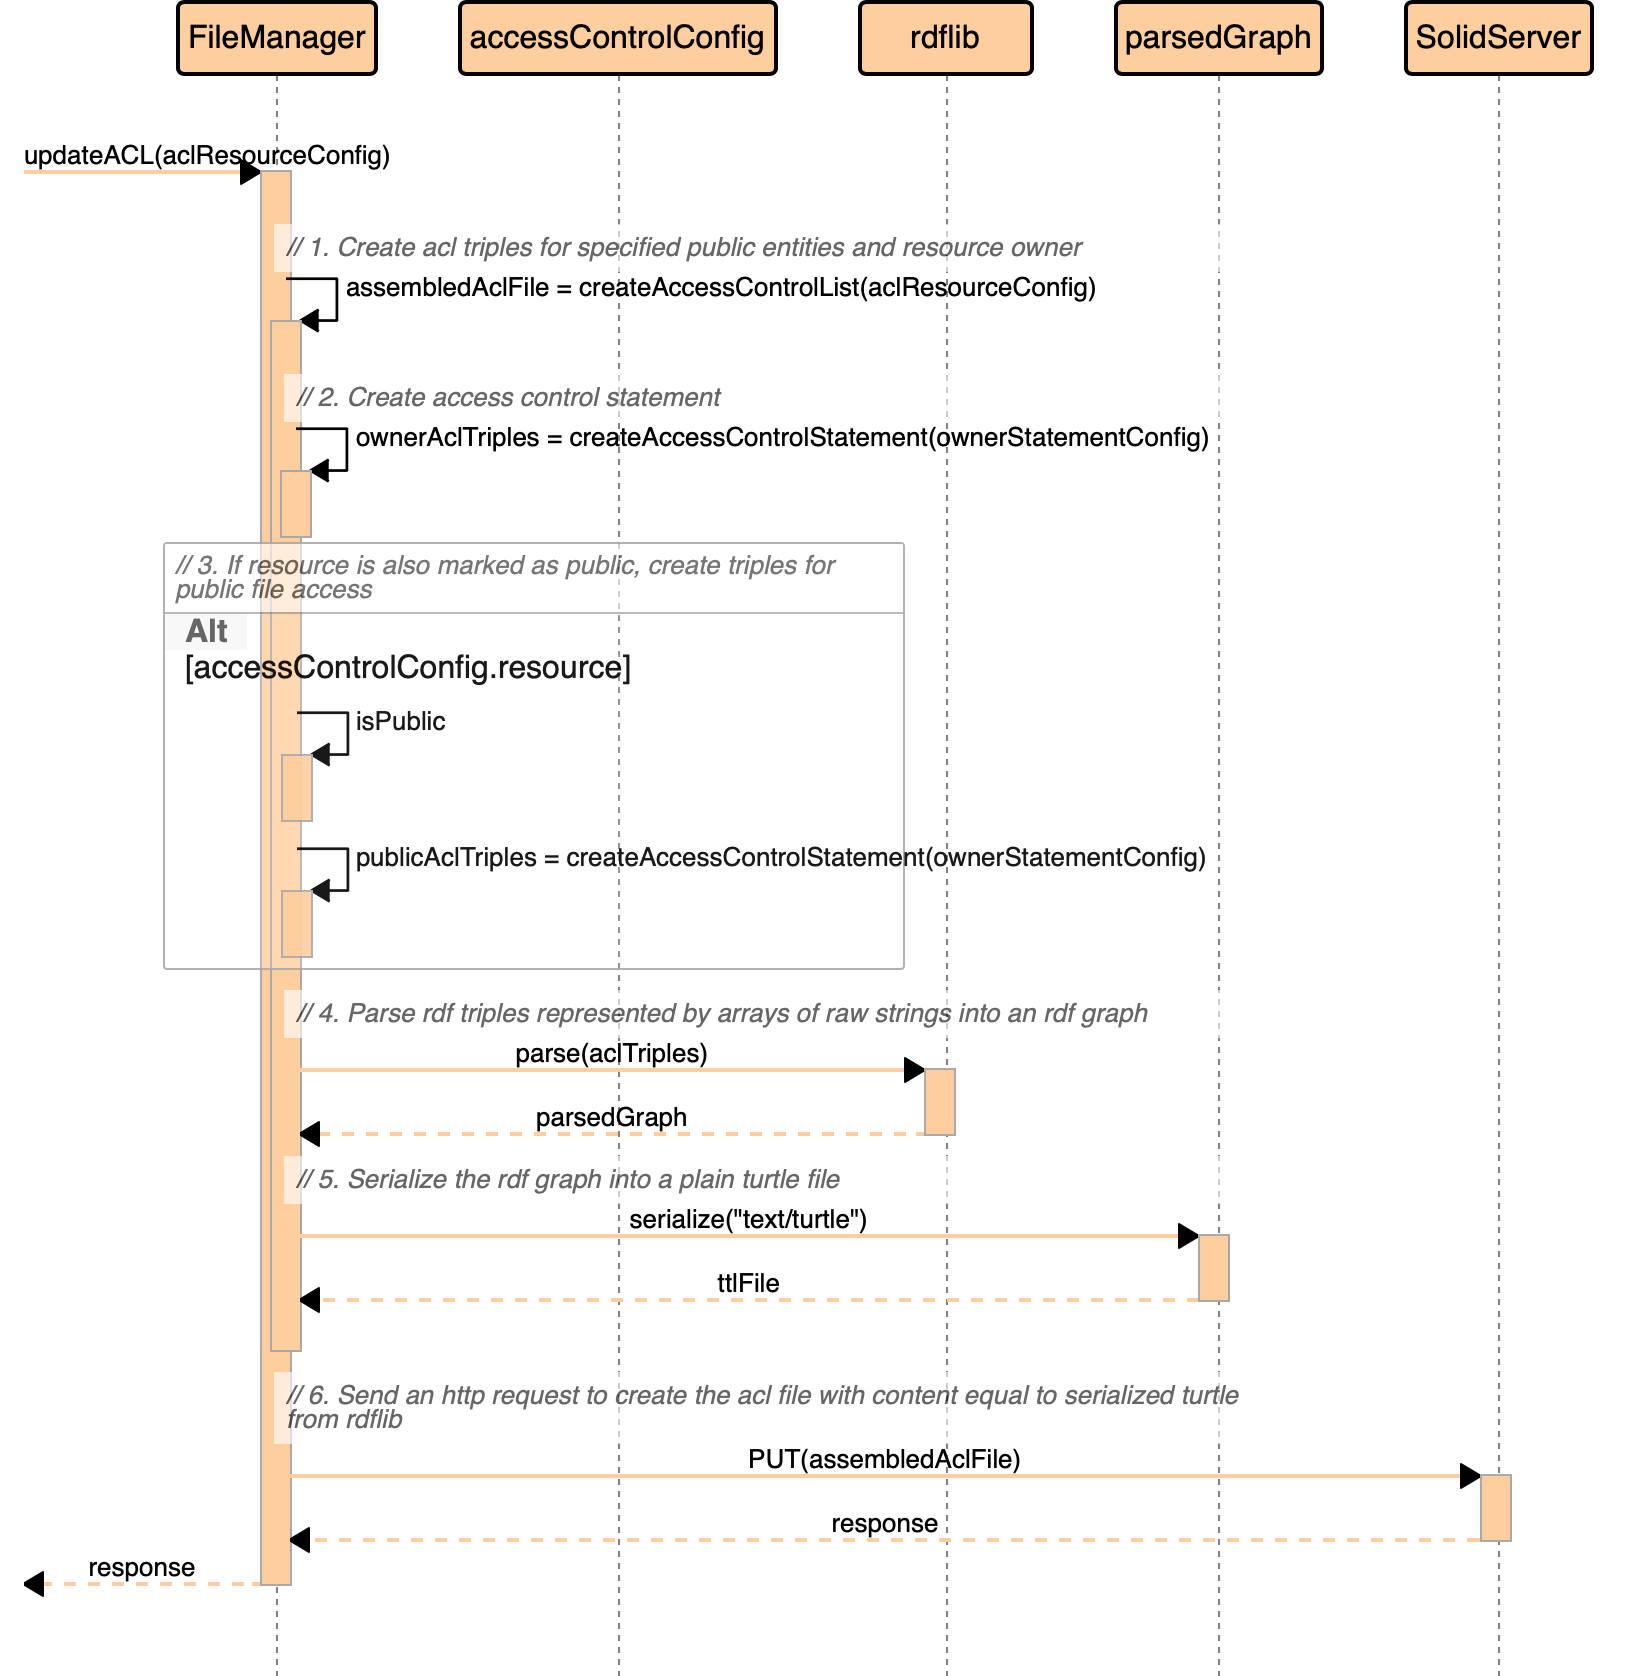
\includegraphics[width=14cm]{acl_update_flow.png}
\caption{A higher level class diagram of classes contained within StorageFileManager abstraction.}
\label{fig:lps_acl_update_flow}
\end{figure}


\section{LinkedPipes Applications vocabulary}

%TODO Add citation to original solid paper
Relying on LDP specification extended by \solid{} was not the only goal while designing an architecture to satisfy the requirements of \lpa{}. It was also important to use advantages of LinkedData in general, and as stated in introductory chapters, as well as the original paper, one the major benefits of any \solid{} compliant server is that everything is either RDF or has the metadata in RDF.  

The first task was to identify and analyze the kind of data that \lpa{} is storing. 

\subsection{Configuration}
\subsubsection{VisualizerConfiguration}
\subsubsection{FilterConfiguration}
\subsubsection{FilterGroup}

\begin{figure}[h]
\centering
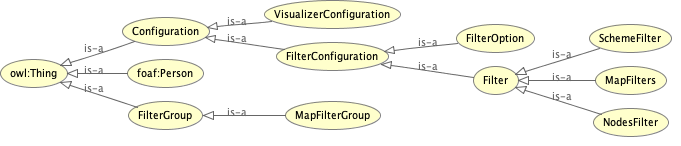
\includegraphics[width=14cm]{lpas_vocabulary_visualization.png}
\caption{A class hierarchy visualization of \lpa{} vocabulary.}
\label{fig:lpas_vocabulary_visualization}
\end{figure}


\begin{figure}[h]
\centering
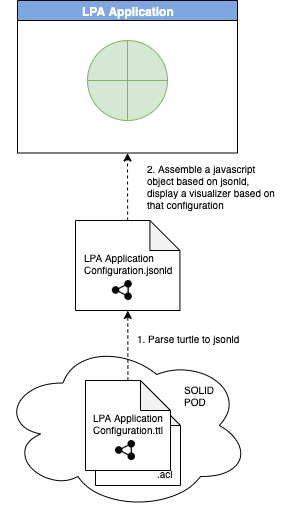
\includegraphics[width=6cm]{lpas_vocabulary_usage.png}
\caption{A formal representation of \lpa{} configurations expressed as RDF files using the \lpas{} vocabulary.}
\label{fig:lpas_vocabulary_usage}
\end{figure}


\section{Storage Component design conventions}


It is important to note that the \lpas{} is not just the external package completely isolated from the \lpa{} frontend, it is also a set of React components that attempt to blend in into the user interface guidelines of the frontend. Now when the major components of the \lpas{} package as well as the \lpas{} vocabulary are described, let us dive deeper into the implementations done on the frontend side inside the \lpa{} codebase. 

The \lpa{} frontend codebase was implemented using React\footnote{https://reactjs.org} and was utilising a modern stack of frontend development tools, all of those had to be taken into consideration to design React Component responsible for interactions with the storage. This section will cover the design conventions inherited from \lpa{} as well as a detailed overview of User Interfaces conforming to Material Design\footnote{https://material.io/design} conventions that were strongly utilized in \lpa{} frontend.  

\subsection{Designing the React component}

At the root, \lpa{} frontend identifies two main types of components that are logically separated into folders titled as follows:
\begin{itemize}
	\item \texttt{Components} folder, these usually contain elements that are used in more than one webpage throughout the project, such as buttons, switches, image wrappers and etc.
	\item \texttt{Containers} folder, represent complex react components that are basically rendering individual webpages or sub-elements of webpages that deal with complex user interaction scenarios.
\end{itemize}

\subsubsection{Simple components}

Whenever an individual component needs to be implemented and it will be used in multiple webpages throughout the project, it is being placed into \texttt{Components} folder.

There are two main types of components that can be placed into \texttt{Components} folder and have different design conventions:
\begin{itemize}
	\item Simple stateless component responsible for plain rendering.
	\item A complex component that needs to aggregate multiple sub-components, manage external state, internal states and etc.
\end{itemize}


This is not a strict guideline defined by \lpa{} developers. However, if a component becomes too complex, as demonstrated on figure \ref{fig:lpas_component_design} the intent is to split component into separate component responsible for rendering and component that manages states of the stateless component. This allows easier navigation within frontend codebase as well as faster code debugging. 

\begin{figure}[h]
\centering
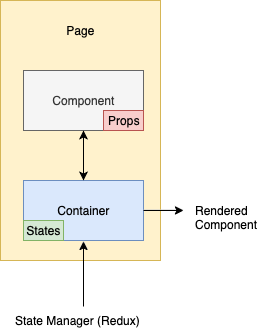
\includegraphics[width=8cm]{lpas_component_design.png}
\caption{React container abstraction decomposition following \lpas{} design conventions.}
\label{fig:lpas_component_design}
\end{figure}

Therefore, this concludes the only major design conventions that were required by \lpa{} frontend. Let us go over the details of each individual component in the following sections.

\subsection{Storage Dashboard}

Referring back to the functional requirements stated in first chapters, the ability to interact with the \lpas{} is an essential feature allowing users of \lpa{} platform to manipulate their Applications. The mock displayed on \ref{fig:lpas_ui_dashboard_mock} is a webpage accessible via the home dashboard. There are two main display modes:

\begin{itemize}
	\item The \textit{My apps} tab, is a React component that fetches all RDF resources in root \lpas{} folder containing applications created by a user. 
	\item The \textit{Shared} tab, is a React component fetching all RDF resources in a shared \lpas{} folder containing applications created and shared by a particular users with other users of \lpas{} platform.
\end{itemize}


\begin{figure}[h]
\centering
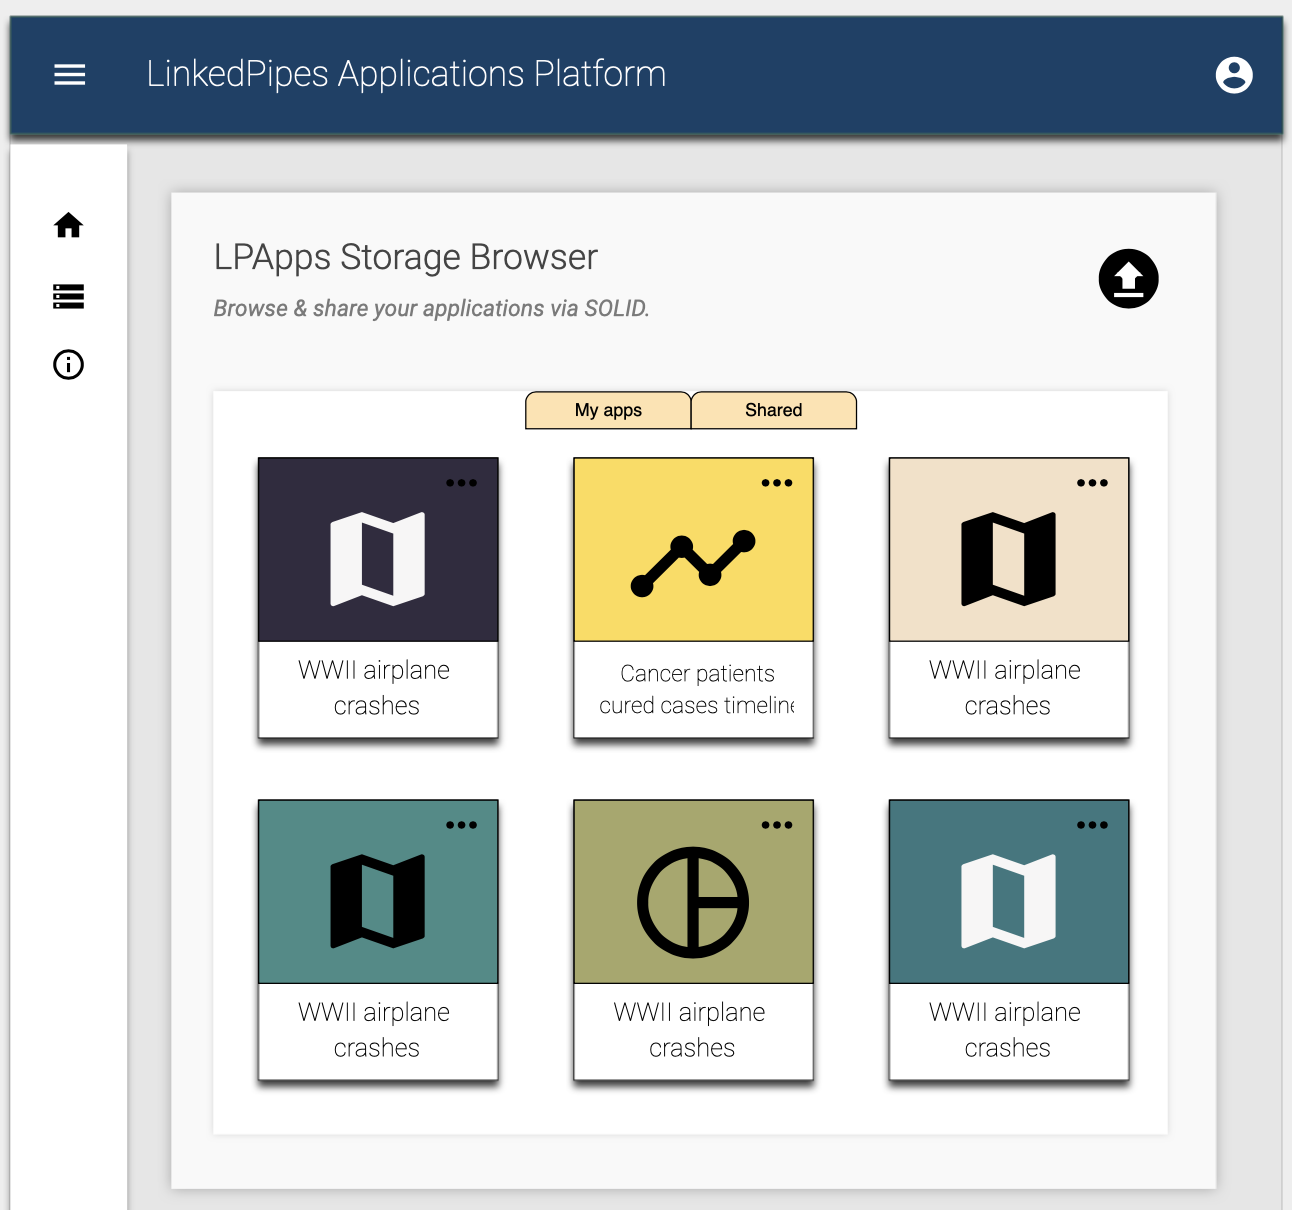
\includegraphics[width=11cm]{lpas_ui_dashboard_mock.png}
\caption{Mock UI for Storage Dashboard webpage in \lpa{} Frontend.}
\label{fig:lpas_ui_dashboard_mock}
\end{figure}

\subsection{Storage Visualizer Preview}


\begin{figure}[h]
\centering
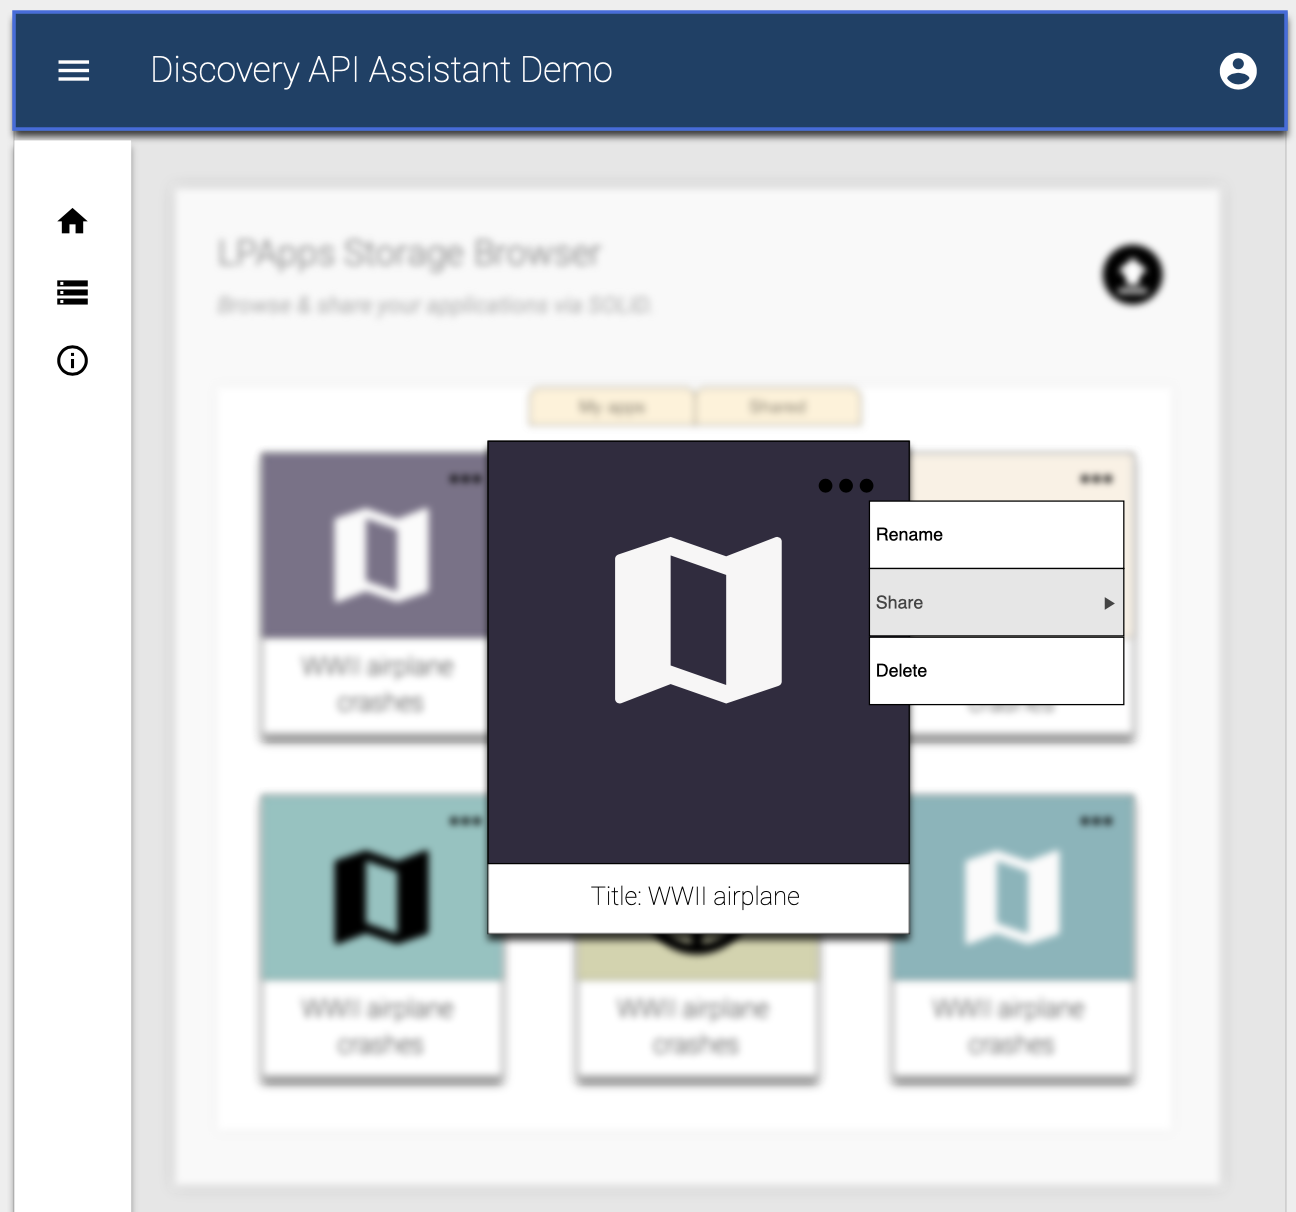
\includegraphics[width=11cm]{lpas_ui_preview_mock.png}
\caption{Mock UI for Visualizer preview popup in \lpa{} Frontend.}
\label{fig:lpas_ui_preview_mock}
\end{figure}
